\section{Why the target is wrong, and a claim we tested and lost}
\label{sec:mechanism}

The transition preserves something, and the previous section shows it is not the optimal readout of
true energy. This section explains why the probe's target was wrong, and then reports a stronger
claim we tested and lost. The explanation is a property of the data and we verify it directly: the
trajectories do not conserve textbook energy, so a probe fitted to textbook energy is fitted to the
wrong quantity. The stronger claim is that the \emph{model} internalised the integrator's quantity.
We designed an experiment that separates model from data, ran it, and it came out negative. We report
it because a reader would otherwise draw the inference we drew. Nothing in
Sections~\ref{sec:dissociation} or~\ref{sec:causality} depends on either.

\paragraph{The data does not conserve textbook energy.}
Trajectories come from semi-implicit (symplectic) Euler,
\begin{equation}
\dot\theta_{n+1} = \dot\theta_n + \tfrac{3g}{2l}\sin(\theta_n)\,\Delta t,
\qquad
\theta_{n+1} = \theta_n + \dot\theta_{n+1}\,\Delta t .
\end{equation}
A symplectic integrator does not conserve the continuous system's Hamiltonian $H$. It conserves a
nearby \emph{shadow} $\tilde H = H + \mathcal{O}(\Delta t)$ \citep{hairer2006geometric}. Here the
first-order correction is $\tfrac{\Delta t}{2}\{T,V\} \propto \dot\theta\sin\theta$, giving
\begin{equation}
\tilde H \;=\; E \;+\; c^\star\,\dot\theta\sin\theta,
\qquad
c^\star \;=\; \tfrac{\Delta t}{2}\,mg\tfrac{l}{2} \;=\; 0.125 ,
\label{eq:shadow}
\end{equation}
with no free parameters. If the model learned the integrator's map rather than the textbook physics,
its transition should preserve $\tilde H$, and a probe fitted to $E$ then has the wrong target
however well it fits.

\paragraph{A sweep, not a two-point test.}
A two-point comparison, a probe fitted to $E$ against one fitted to $\tilde H$, would not settle
this: $\tilde H$ is a different function, and its advantage could come from being easier to
represent. We therefore sweep the family
\begin{equation}
T_c(\theta,\dot\theta) \;=\; E(\theta,\dot\theta) \;+\; c\,\dot\theta\sin\theta ,
\end{equation}
over a grid that contains $c^\star$, both signs, and wrong magnitudes $2\times$ and $4\times$ either
way, refitting at each $c$ with everything else held fixed. At $c=0$ the sweep reduces to the
supervised probe of Section~\ref{sec:dissociation} and reproduces its numbers to five decimals. The
prediction is the location of a minimum, which no representational-ease artifact produces, and we
registered it before the sweep ran.


\begin{figure}[t]
\centering
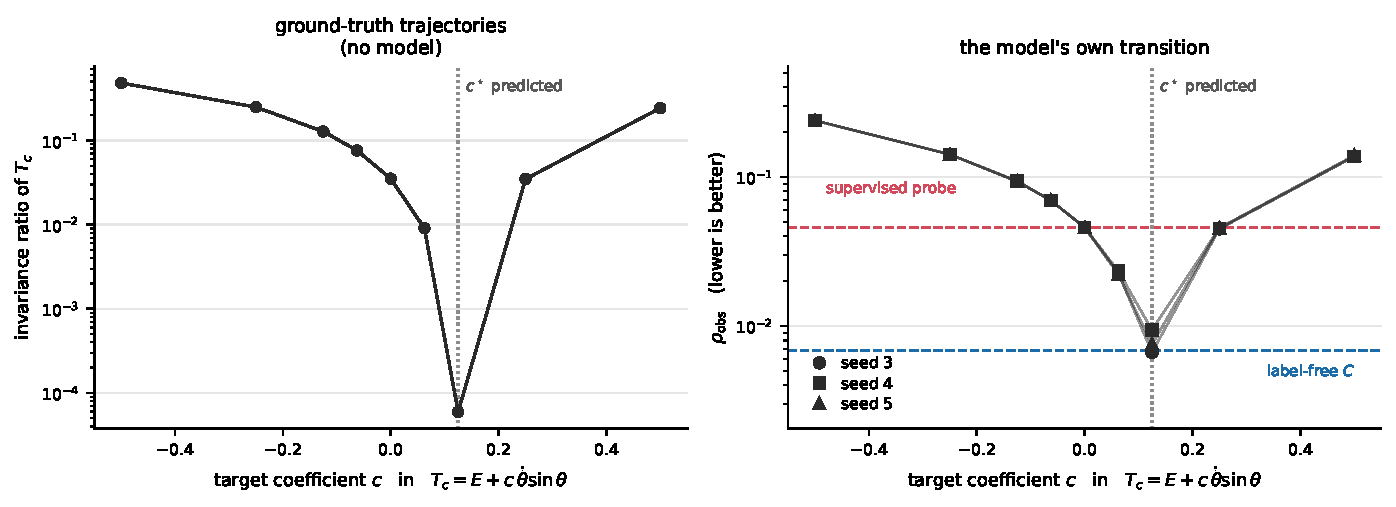
\includegraphics[width=\textwidth]{figures/fig2_shadow_sweep.pdf}
\caption{The model's transition conserves the integrator's shadow Hamiltonian, not textbook energy.
Both panels sweep the target $T_c = E + c\,\dot\theta\sin\theta$; the dotted line is $c^\star = 0.125$
predicted from the integrator with no fitting. \textbf{Left:} on ground-truth trajectories, with no
model involved, $T_{c^\star}$ is $591\times$ better conserved than textbook energy. \textbf{Right:}
the learned transition agrees, on all three seeds. The sweep passes from the supervised probe's level
(red) down to the label-free scalar's (blue) exactly at $c^\star$. The wrong-sign control at
$c=-c^\star$ is $12\times$ worse (median over seeds), so this is not monotone in $|c|$.}
\label{fig:shadow}
\end{figure}

\paragraph{The minimum is where the integrator says it is.}
Figure~\ref{fig:shadow} shows both halves. On ground-truth trajectories, with no model involved, the
invariance ratio of $T_c$ falls by $591\times$ between $c=0$ and $c=c^\star$, which confirms the
derivation and fixes the sign. On the learned transition, $\rho_{\mathrm{obs}}$ reaches its minimum
at $c^\star$ on 3 of 3 models, falling $4.9$--$6.9\times$ below its value at $c=0$. The curve is
not monotone in $|c|$: the wrong-sign, right-magnitude control at $c=-c^\star$ is $12\times$ worse
than at $c=+c^\star$ (range $10$--$14\times$ over the three models). A post-hoc refinement over
$c \in [0.090, 0.170]$ locates the minimum at $0.125 \pm 0.005$ on every seed.

The repair follows the same curve. Enforcing $T_{c^\star}$ during imagination changes energy drift by
$-49.5\%$, $-31.5\%$ and $-29.3\%$ on the three models, a repair on all three, while enforcing
$T_0$, the perfect probe, gives $+26.8\%$, $-0.3\%$ and $+33.4\%$. Correcting an
$\mathcal{O}(\Delta t)$ term in the target flips the intervention from harmful to helpful.

\paragraph{The coefficient tracks the simulator's timestep on the evaluation data.}
If the model has learned the integrator rather than the physics, $c^\star$ is a property of the
discretisation and not a constant of the pendulum, so changing the simulator's timestep should move
it: $c^\star(\Delta t) = \tfrac{\Delta t}{2}mg\tfrac{l}{2} = 2.5\,\Delta t$. We test this directly,
generating four datasets at $\Delta t \in \{0.02, 0.035, 0.05, 0.08\}$ that are identical in every
other respect and training three models on each. We express the sweep relatively,
$r = c/2.5\Delta t$, so the prediction is a single value of $r$ at every timestep.

\begin{table}[t]
\centering\small
\caption{The recovered correction tracks the simulator's timestep across a $4\times$ range. Three
models per timestep; $\rho_{\mathrm{obs}}$ is the median across seeds.}
\label{tab:timestep}
\begin{tabular}{lccccc}
\toprule
$\Delta t$ & predicted $c^\star$ & $\arg\min_r$ per seed & $\rho_{\mathrm{obs}}$ at $r{=}0$ & at $r{=}1$ & separation \\
\midrule
0.02  & 0.050 & $+0.75,+0.75,+1.00$ & 0.0171 & 0.0166 & 1.03$\times$ \\
0.035 & 0.088 & $+1.00\times3$ & 0.0231 & 0.0103 & 2.24$\times$ \\
0.05  & 0.125 & $+1.00\times3$ & 0.0449 & 0.0079 & 5.72$\times$ \\
0.08  & 0.200 & $+1.00\times3$ & 0.1188 & 0.0088 & \textbf{13.5}$\times$ \\
\bottomrule
\end{tabular}
\end{table}

Table~\ref{tab:timestep} shows the outcome. The minimum sits exactly at the predicted $r=1$ on 10 of
12 models, and the models beat the wrong-sign control on 12 of 12. We regress the recovered
coefficient on $\Delta t$ through the origin, as the theory requires, and get a slope of
$2.484 \pm 0.058$ against a parameter-free prediction of $2.500$, agreement to $0.6\%$ with nothing
fitted.

Two scalings make the mechanism visible. As the timestep coarsens, $\rho_{\mathrm{obs}}$ for textbook
energy grows as $\Delta t^{1.41}$, while $\rho_{\mathrm{obs}}$ for the shadow quantity stays at the
model's own floor, $0.008$--$0.017$ across the whole range. The separation between them therefore
grows from $1.03\times$ to $13.5\times$, purely because textbook energy becomes worse conserved while
the shadow quantity does not. At every timestep, the quantity best conserved along these trajectories
is the integrator's rather than the physicist's.

We report one registered failure. Our preregistration required a slope within $20\%$ and an intercept
whose interval contains zero; the two-parameter fit gives a slope of $2.611 \pm 0.110$ but an
intercept of $-0.0072 \pm 0.0057$, which excludes zero. The smallest timestep drives it entirely, and
a post-hoc finer grid puts the minimum there at $r = 0.875$ on all three seeds, a real $12\%$ low
bias rather than grid coarseness. That is the regime where the whole separation is only $1.03\times$
and the residual curve is flat to within $2\%$.

\paragraph{The model does not track the timestep.}
Table~\ref{tab:timestep} is a statement about the data with the model in the loop, and the two cannot
be separated by varying the data alone. Our statistic $\rho_{\mathrm{obs}}$ measures how well a
candidate is conserved along given trajectories, so both the checkpoint and the evaluation set
influence the argmin. A registered cross-evaluation control shows which dominates: crossing models
against datasets, the argmin follows the \emph{evaluation set} in all six cells and the checkpoint in
none.

The decisive experiment holds the data fixed instead. We trained three models with $\Delta t$
supplied in a conditioning channel, evaluated every one on a single fixed dataset, and swept only the
value we told the model. A model that has internalised the integrator's coefficient should move its
argmin with the conditioning; a model reading the data should not. The models demonstrably use the
channel: shuffling it degrades one-step prediction on $3/3$ seeds against a preregistered bar. The
argmin nevertheless moves by $+0.0125$ against a predicted $+0.1500$, a tracking fraction of
$0.074$, $0.074$ and $0.111$. The coefficient is about $93\%$ a property of the data the statistic is
computed on. \textbf{The model does not carry the integrator's timestep, and we report the claim as
falsified rather than open.}

We also record that two of our own registered predictors passed on this experiment and both were
wrong. A rank correlation is scale-free, so an $8\%$ move scores $1.0$ when it is monotone, and a
slope band cannot separate the hypotheses because a constant argmin at the data's value scores
$2.197$ against perfect tracking's $2.500$. The tracking fraction above is sensitive to magnitude,
which is the entire question. A companion attempt to identify the integration \emph{scheme} is
unfalsifiable rather than false: semi-implicit Euler and velocity Verlet reduce to the identical
position recurrence $\theta_{t+1} = 2\theta_t - \theta_{t-1} + a(\theta_t)\Delta t^2$, differing only
in whether $\dot\theta$ carries a backward or a central difference, which the pixels never show.

\paragraph{What survives.}
The data-side explanation stands and is what the dissociation needs. On ground truth the trajectories
conserve the quantity at the integrator's predicted coefficient $591\times$ better than textbook
energy, with nothing fitted, and correcting that $\mathcal{O}(\Delta t)$ term flips the intervention
from harmful to repairing on every model. A probe fitted to true energy is therefore fitted to a
quantity \emph{the generating process does not conserve}, and no probe hygiene detects this, because
nothing is wrong with the probe. The target is.

The residual is worth recording: median $\rho_{\mathrm{obs}}$ at $c^\star$ is $7.5\times10^{-3}$
against the label-free scalar's $6.9\times10^{-3}$, a gap of $1.10\times$, so the shadow quantity
accounts for essentially all of the gap in Section~\ref{sec:dissociation}. The sweep is also
internally decisive about the probing point, and needs no model-versus-data attribution: at $c^\star$
the readout correlates with textbook energy \emph{worse} than at $c=0$ ($0.977$ against $0.9999$)
while being conserved six times better and repairing the rollout instead of harming it. Correlation
with the labelled quantity and fitness for the dynamics move in opposite directions along a single
one-parameter family. The label-free method's advantage does not depend on this section either: it
optimises conservation under the learned transition, so it is not restricted to targets a human knows
how to write down, and here it recovered an $\mathcal{O}(\Delta t)$ correction nobody supplied.
